\chapter{SYSTEM DESIGN}

\section{Requirement Specification}

\subsection{Functional Requirements}
\begin{itemize}
    \item \textbf{Input Handling:} The system accepts handwritten Nepali word images from the IIIT-HW-Dev dataset during training and evaluation, as well as user-provided images during inference.

    \item \textbf{Image Pre-processing:} Input images are automatically passed through a multi-step pipeline comprising grayscale conversion, denoising, adaptive binarisation, morphological closing, deskewing, tight cropping, and letterbox padding to $128 \times 128$ pixels, followed by rescaling to $384 \times 384$ pixels and normalisation by the ViTImageProcessor to match the ViT encoder's pre-training distribution.

    \item \textbf{Feature Extraction and Recognition:} The pre-trained ViT encoder extracts a contextual visual feature matrix from the input image, and the custom BERT-based decoder  attends to these features via cross-attention to autoregressively generate the corresponding Nepali Unicode word.

    \item \textbf{Tokenization:} A custom character-level tokenizer encodes ground-truth Unicode labels into integer token sequences and decodes predicted token IDs back into Devanagari text using a 112-token vocabulary.

    \item \textbf{Training and Evaluation:} The system is trained using label-smoothed cross-entropy loss and evaluated using Character Error Rate (CER), Word Error Rate (WER), Exact Match Accuracy, and Normalised Edit Distance (NED).

    \item \textbf{Inference:} The model generates predictions using beam search decoding (num\_beams = 4)), returning the top 3 candidate transcriptions ranked by sequence log-probability score.

    \item \textbf{Output:} The primary output is the highest-scoring candidate Nepali word in Unicode format. For single-image inference, two additional confidence signals are reported:
\begin{enumerate}
    \item Per-character confidence, expressed as a percentage derived from 
    per-token transition probabilities.
    \item Sequence-level beam scores (log-probability) for each of the top 
    3 alternative predictions, allowing the user to assess and manually 
    select a more appropriate candidate if needed.
\end{enumerate}
\end{itemize}

\subsection{Non-Functional Requirement}
\begin{itemize}
    \item \textbf{Performance:} The system should provide accurate predictions with reasonable response time using GPU acceleration.

    \item \textbf{Scalability:} The model can be extended to process full sentences or paragraphs by adding a word segmentation module.

    \item \textbf{Accuracy:} The system aims to achieve low CER and WER, and high Exact Match Accuracy on the test dataset.

    \item \textbf{Usability:} The model should be easy to use and deploy as a standalone tool or API for digitizing handwritten documents.

    \item \textbf{Reliability:} The system should produce consistent results across different handwriting styles.
\end{itemize}
\newpage
\section{Use Case Diagram}
      The Use Case Diagram \ref{fig:use case diagram} illustrates the interaction between the actor and the Nepali Handwritten Word Recognition System.
    \begin{figure}[H]
        \centering
        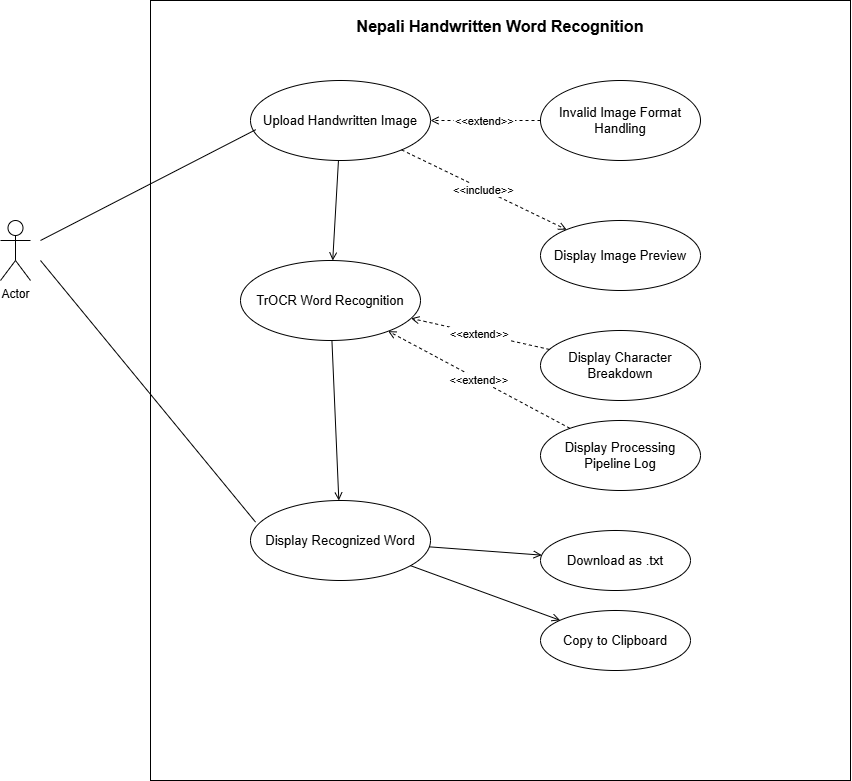
\includegraphics[scale=0.5]{img/UCD.png}
        \caption{Use Case Diagram of Nepali Handwritten Word Digitization}
        \label{fig:use case diagram}
   \end{figure}
     \noindent The process begins when the user uploads a handwritten image, which automatically includes displaying an image preview and may extend to handle invalid image formats. The uploaded image is directly passed into the TrOCR Word Recognition process, which may optionally extend to display a character breakdown. Finally, the recognized word is displayed to the user, with additional options to download the result as a .txt file or copy it to the clipboard.
%\section{Activity Diagram}
   % \begin{figure}[H]
      %  \centering
        %\includegraphics[scale=0.69]{img/ActivityDiagram.png}
       % \caption{Activity Diagram}
       % \label{fig:activity diagram}
  % \end{figure}
 %  The activity diagram illustrates the complete workflow of the system from start to finish. The process begins when the user uploads a handwritten image. If the image format is invalid, an error message is displayed and the process terminates. If the format is valid, the image preview is shown and the image enters the preprocessing pipeline, which consists of grayscale conversion, binarization, deskewing, and tight cropping. The preprocessed image is then fed into the fine-tuned TrOCR model to generate Unicode Nepali text. The post-processing stage runs in parallel to display the recognized word, generate a character-level confidence breakdown, and produce a pipeline processing log. Finally, if the user chooses to export the result, they can either download it as a .txt file or copy it to the clipboard, after which the process ends.

\newpage
\section{Class Diagram for System}
This class diagram \ref{fig:classdiagram} illustrates the structure of the Nepali Handwritten Word Recognition System.
\begin{figure}[H]
    \centering
    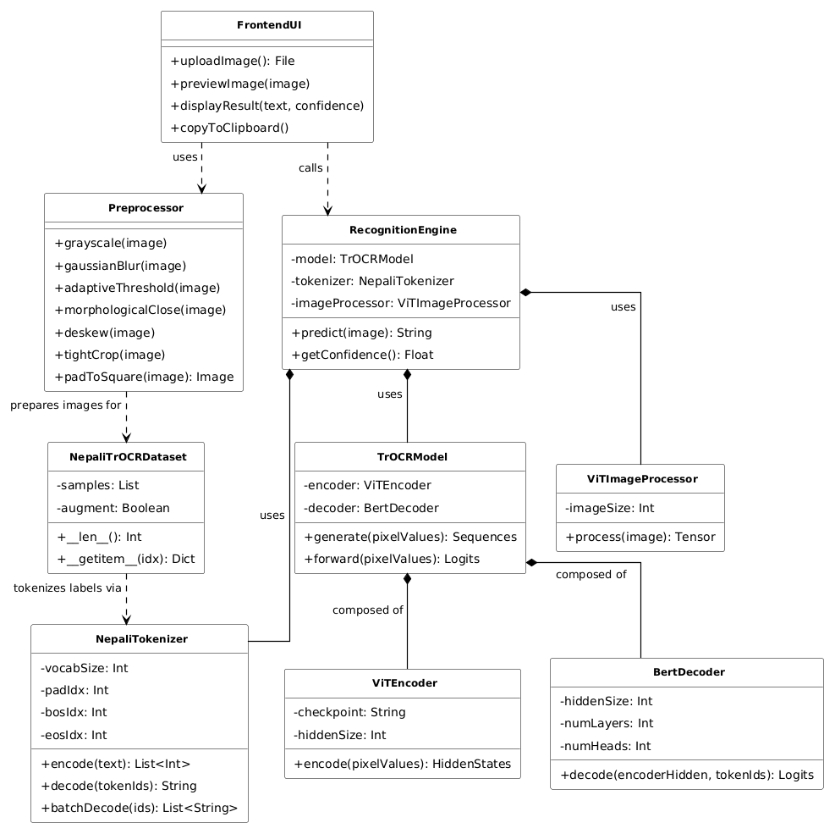
\includegraphics[width=\textwidth]{img/ClassDiagram.png}
    \caption{Class diagram of Nepali Handwritten Word Digitization}
    \label{fig:classdiagram}
\end{figure}
 \noindent The FrontendUI is the entry point where the user uploads a handwritten word image and receives the predicted text with confidence scores. It directly interacts with the Preprocessor, which cleans the image through a seven-step pipeline, and the RecognitionEngine, which handles inference. The preprocessed images feed into the NepaliTrOCRDataset, which uses the NepaliTokenizer to convert Devanagari labels into character-level token IDs. During inference, the RecognitionEngine coordinates the TrOCRModel, NepaliTokenizer, and ViTImageProcessor. The TrOCRModel is composed of a pretrained ViT encoder and a lightweight custom BERT-based decoder consisting of two layers, four attention heads, hidden size 256 to generate the recognised character sequence. Each class has a single well-defined responsibility, ensuring a clean data flow from raw handwritten input to Unicode text output.



  
%\section{Class Diagram for Data }

%\section{Database Schema}

\section{Sequence Diagram}
The sequence diagram \ref{fig:sequence diagram} depicts the step-by-step interaction between the system components during a recognition request. The user uploads a handwritten image through the Frontend UI, which previews the image before the user initiates recognition. The frontend sends a POST request to the FastAPI Backend, which forwards the image to the Preprocessor. The Preprocessor applies grayscale conversion, binarization, deskewing, and tight cropping before returning the cleaned image to the backend.
    \begin{figure}[H]
        \centering
        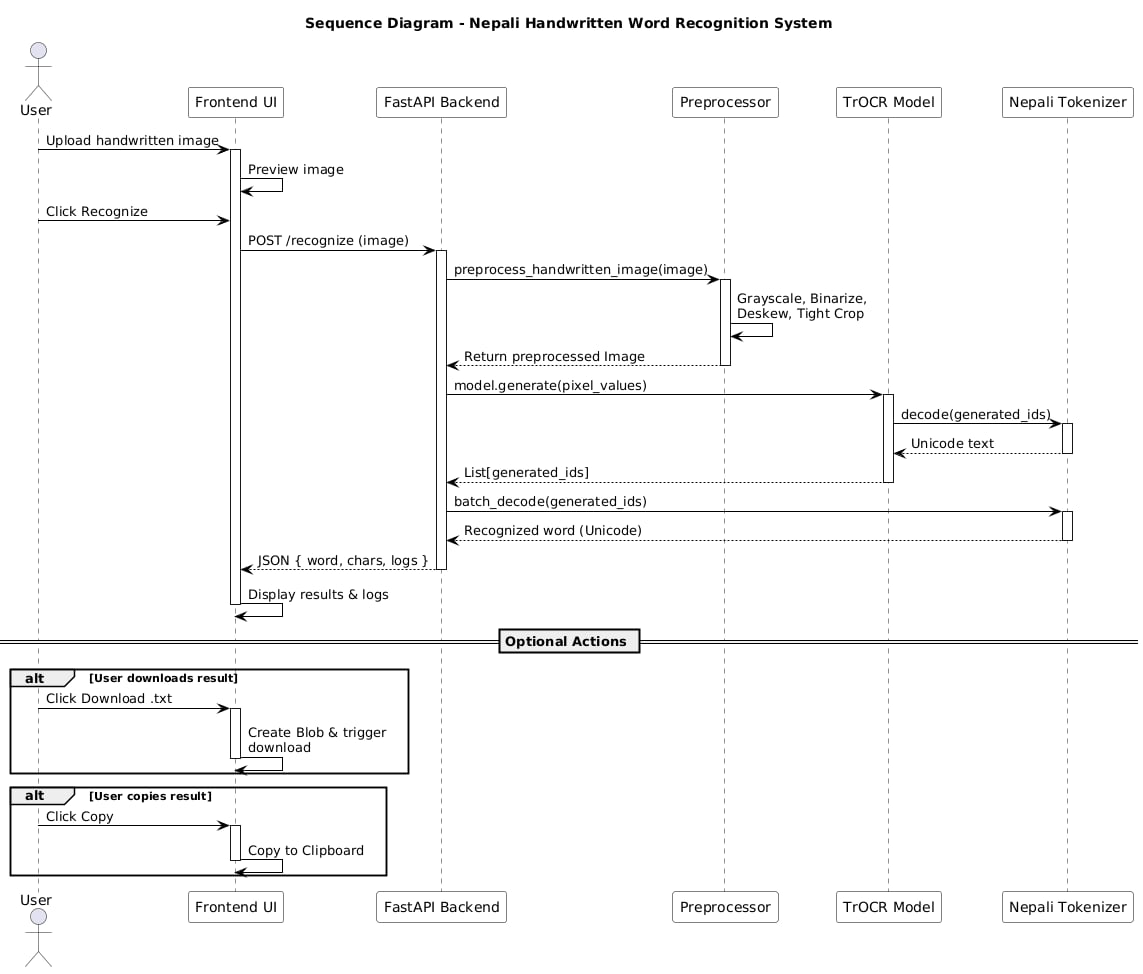
\includegraphics[scale=0.4]{img/SD.jpg}
        \caption{Sequence Diagram of Nepali Handwritten Word Digitization}
        \label{fig:sequence diagram}
   \end{figure}
   \noindent The backend then calls the TrOCR Model to generate token IDs, which are decoded into Unicode text by the Nepali Tokenizer. The final recognized word is returned to the frontend as a JSON response and displayed to the user. Optionally, the user may download the result as a .txt file or copy it to the clipboard.

%\section{Data Flow Diagram}

   % \begin{figure}[H]
      %  \centering
       % \includegraphics[scale=0.38]{img/dfd0.png}
       % \caption{Level 0 Data Flow Diagram}
       % \label{fig:Level 0 Data Flow Diagram}
  % \end{figure}
  % The context diagram provides a high-level overview of the system. The user provides a handwritten image as input to the Nepali Handwritten Word Recognition System. The system processes the image and returns the recognized Unicode Nepali text, downloadable output, and confidence logs back to the user. Any invalid image format triggers an error notification.

   % \begin{figure}[H]
      %  \centering
       % \includegraphics[scale=0.5]{img/Level1.jpg}
      %  \caption{Level 1 Data Flow Diagram}
       % \label{fig:Level 1 Data Flow Diagram}
   %\end{figure}
%\noindent
%The Level 1 Data Flow Diagram breaks down the internal processes of the system. The user submits a handwritten image which enters the Upload Image process. The raw image is then passed to the Preprocess Image process where it is cleaned and normalized. The cleaned image is fed into the Run TrOCR Inference process, which loads model weights from the TrOCR Model data store. The generated token IDs are passed to the Decode Output process, which references the Nepali Tokenizer data store to map tokens to Unicode characters. The resulting Unicode text is then passed to the Display Result process, which returns the recognized word and character breakdown to the user.





%\section{Deployment Diagram}
%\textbf{Note: All the diagram is not mandatory..select according to the type of project you are going to do.}